\documentclass[../Main.tex]{subfiles}
\begin{document}
\chapter{Digital Business}

\intro{

}

\begin{figure}[H]
    \centering
    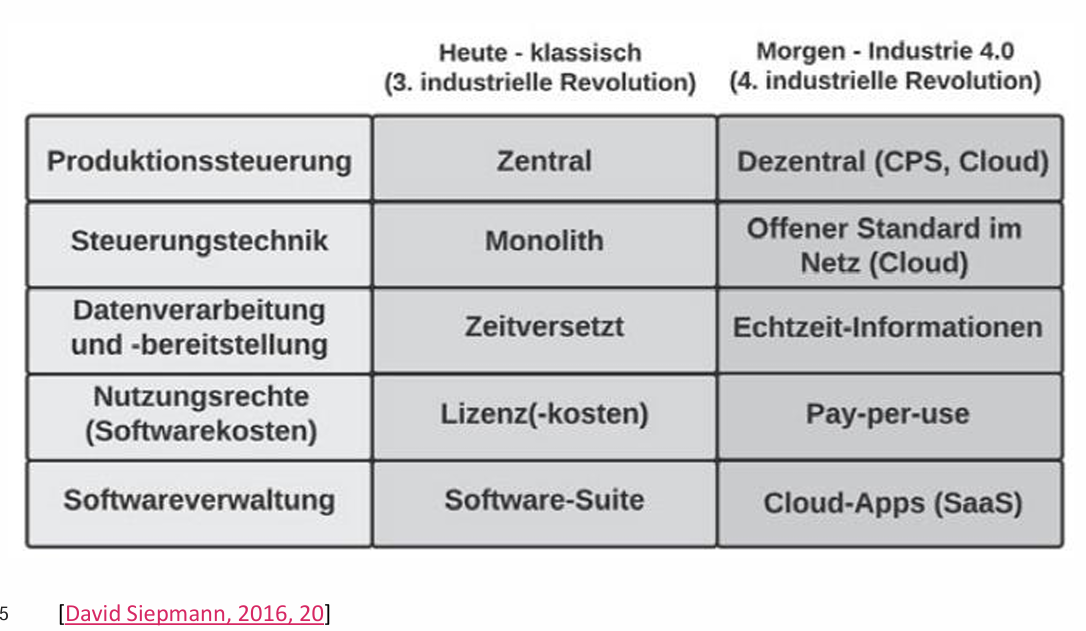
\includegraphics[width=1\linewidth]{Images/digbus/paradigmen-wechsel.png}
    \caption{Paradigmen Wechsel}
\end{figure}

\begin{figure}[H]
    \centering
    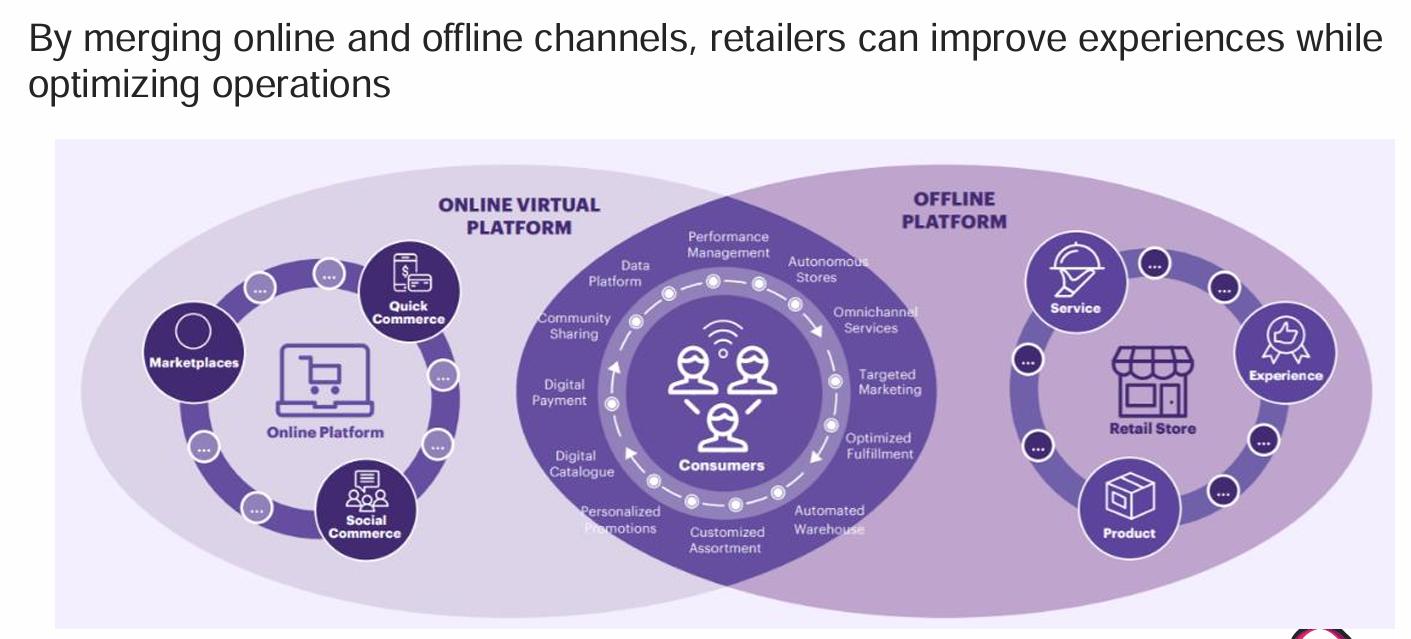
\includegraphics[width=1\linewidth]{Images/digbus/omo.png}
    \caption{Online-Merge-Offline (OMO) im Retail}
\end{figure}

\subsection{Smart Store}
Zeichnet sich aus durch:
\begin{itemize}
    \item Personalisierte Erlebnisse 
    \item Automatisierte Prozesse
    \item IoT
    \item Zahlungsmöglichkeiten ohne Kasse
    \item Verbesserte Logistik und Bestandesverwaltung
    \item Kundensupport und Interatkionen: Chatbots, digitale Assistenten
\end{itemize}

Dimensionen eines Smart Stores:
\begin{itemize}
    \item Wer (Wer profitiert Kunde, Mitarbeiter)
    \item Was (Betrifft front (Kundenerlebnis) oder backend)
    \item Wo (physisch, hybrid, online)
\end{itemize}

Neue Technologien im Retail:
\begin{itemize}
    \item Läden ohne Personal
        \begin{itemize}
            \item Avec Box
            \item Migros Teo
            \item Amazon Go
        \end{itemize}
    \item Electronic Self Label (ESL): Migros
    \item Der invisible Checkout Prozess von Post Finance
\end{itemize}

\subsection{Banking}
\defn{Open Banking}{
    \begin{itemize}
        \item Nach dem Open-Banking-Konzept können Endkunden ihre persönlichen 
        Finanzdaten über offene Schnittstellen verschiedenen Banken bzw. 
        Finanzdienstleistern oder FinTech-Unternehmen zugänglich zu machen. 
        \item Grundlagen von Open Banking bilden technische Schnittstellen (API, SOA) 
        sowie regulatorische Vorgaben (PSD 2).
        \item Open Banking erleichtert die Bildung digitaler Ökosysteme und reduziert die 
        Eintrittsbarrieren für Startup- und Nichtbank-Unternehmen (FinTech, Banking
        Innovation).
    \end{itemize}
}

\begin{figure}[H]
    \centering
    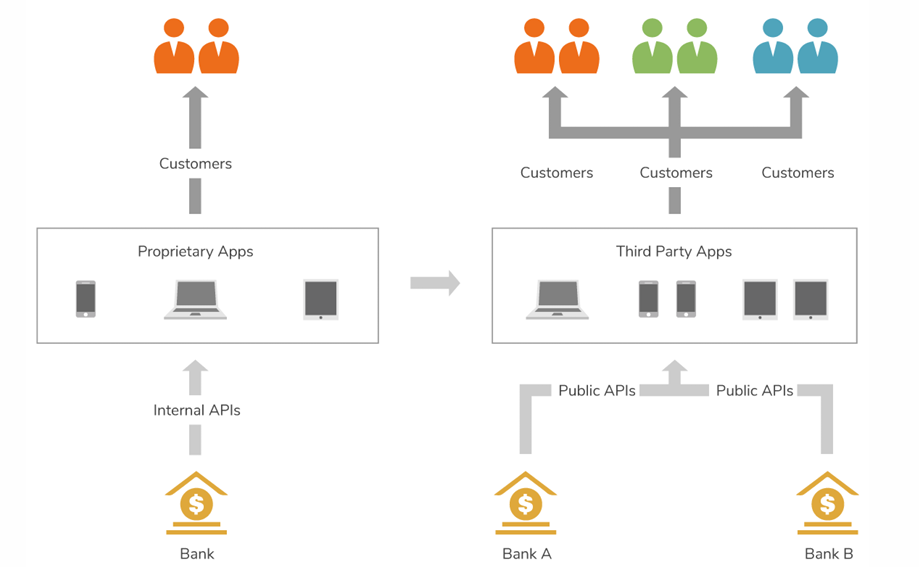
\includegraphics[width=1\linewidth]{Images/digbus/openbanking.png}
    \caption{Open Banking: BaaS/API-Banking}
\end{figure}
\begin{figure}[H]
    \centering
    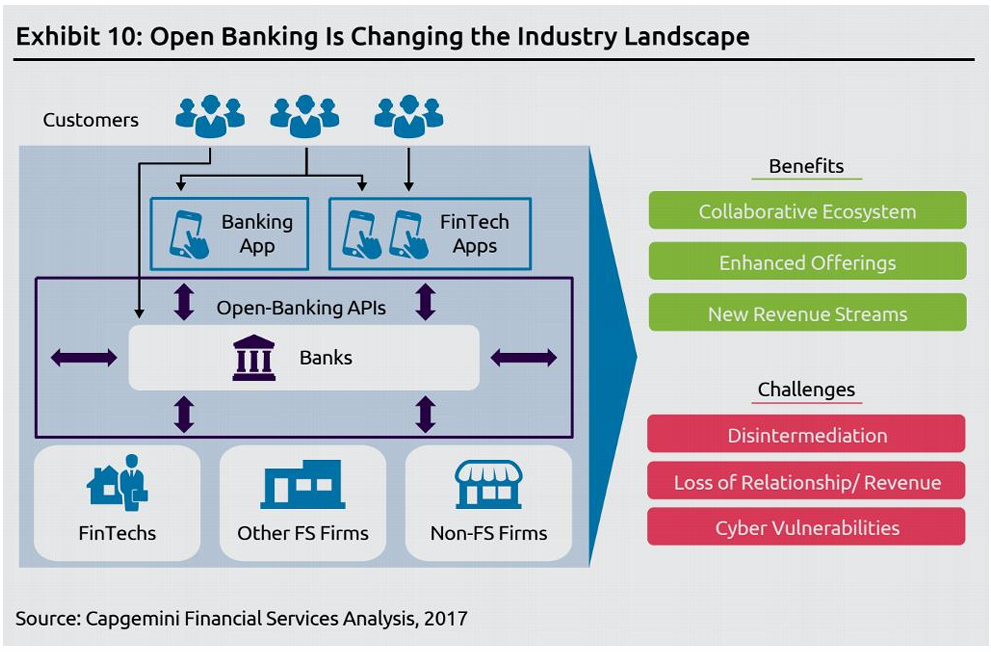
\includegraphics[width=1\linewidth]{Images/digbus/baas.png}
    \caption{Open Banking: Vorteile Nachteile}
\end{figure}

Beispiele:
\begin{itemize}
    \item Avaloq One
    \item Finnova Open Plattform
    \item Hypothekarbank Lenzburg
    \item Swisscom Open Banking Hub
    \item b.Link von Six
\end{itemize}

\begin{figure}[H]
    \centering
    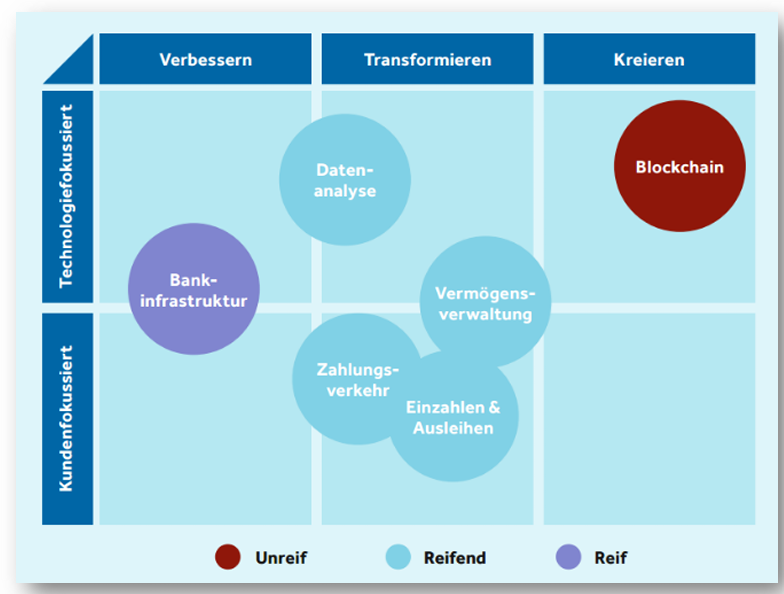
\includegraphics[width=1\linewidth]{Images/digbus/fintech.png}
    \caption{Fintech Sektor}
\end{figure}

\subsection{Industrie 4.0}

\begin{figure}[H]
    \centering
    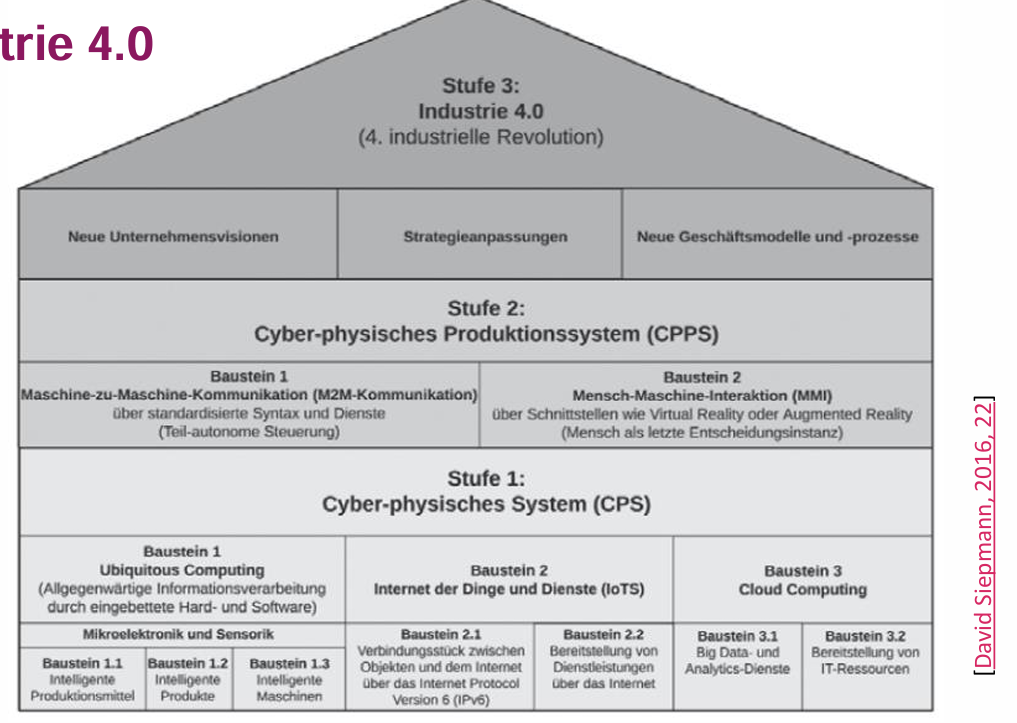
\includegraphics[width=1\linewidth]{Images/digbus/40elemente.png}
    \caption{Komponenten von Industrie 4.0}
\end{figure}

\defn{Smart-Factory}{
    «In einer sogenannten Smart Factory werden die oben beschriebenen Konzepte der Industrie 4.0 
umgesetzt. 
Der Begriff Smart Factory (intelligente Fabrik) bezeichnet eine Fertigung, bei der sich Fertigungs
maschinen und interne Logistik dezentral selbst steuern, indem Maschinen beziehungsweise 
Roboter, Produkte, Werkstücke und Mitarbeiter miteinander digital kommunizieren. 
Intelligente Produkte oder Bauteile sind eindeutig identifizierbar, jederzeit lokalisierbar und 
steuern sich gegebenenfalls autonom durch das Produktionssystem. 
Im Kern handelt es sich um selbststeuernde Prozesse, bei denen die Werkstücke ihre 
fertigungsrelevanten Informationen (aktueller Bearbeitungsstatus, Arbeitsgänge je Maschine, 
alternative Wege zum Zielzustand etc.) mit sich oder auf einem begleitenden Werkstück-Träger 
führen. Anhand dieser Informationen steuert sich das Werkstück (Produkt) autonom durch die 
einzelnen Bearbeitungsstufen des Produktionssystems. 
Das Konzept der Smart Factory geht weit über die traditionelle Automatisierung, bei der etwa ein 
Produktionsplanungs- und Steuerungssystem (PPS) mit der SPS (speicherprogrammierbare 
Steuerung) einer Fertigungsmaschine kommuniziert, hinaus.
}

\begin{figure}[H]
    \centering
    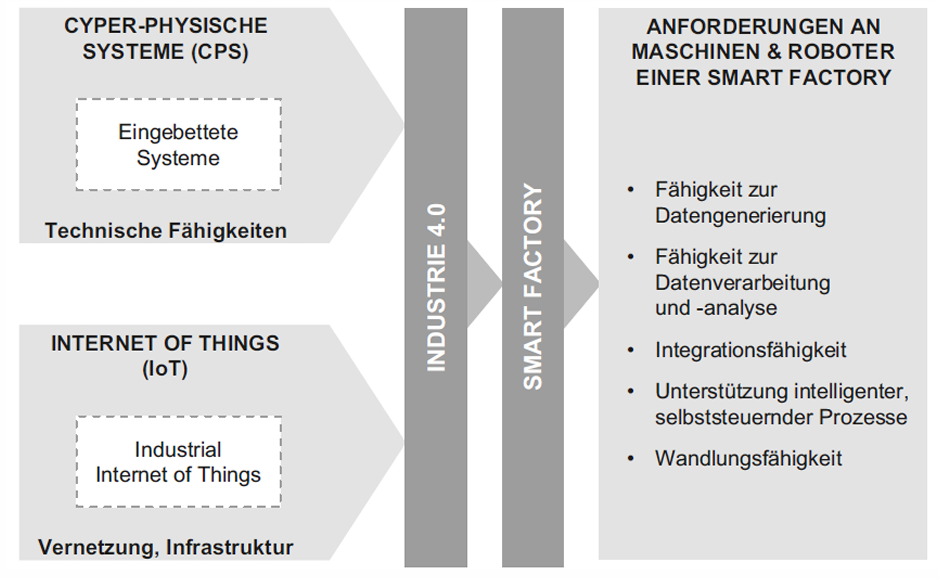
\includegraphics[width=1\linewidth]{Images/digbus/sf.png}
    \caption{Rahmen von Smart-Factory}
\end{figure}

\begin{figure}[H]
    \centering
    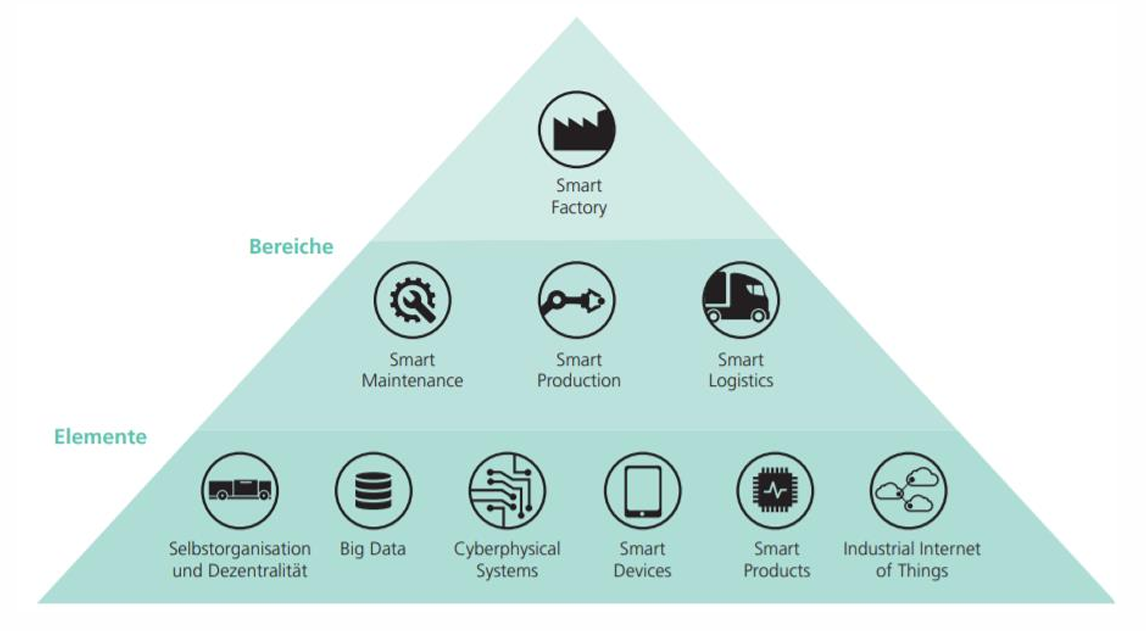
\includegraphics[width=1\linewidth]{Images/digbus/sfbereiche.png}
    \caption{Bereiche einer Smartfactory}
\end{figure}

\begin{figure}[H]
    \centering
    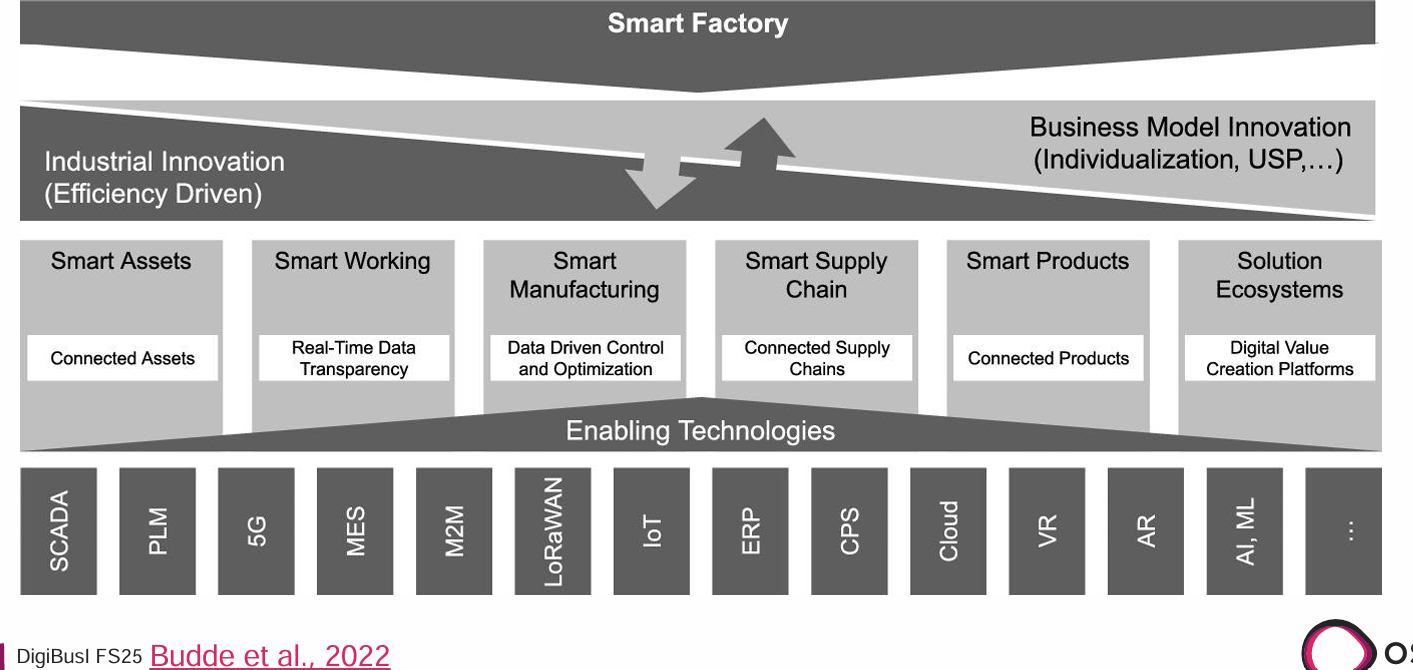
\includegraphics[width=1\linewidth]{Images/digbus/sfdimensionen.png}
    \caption{Dimensionen einer itelligenten Fabrik}
\end{figure}

\section{Digitale Wertschöpfungskette}
Wichtige Dimensionen im Digital Economy:
\begin{itemize}
    \item Wertschöpfungsstrukturen
    \item Wertschöpfungsprozesse
    \item Produkte und Services
    \item Infrastrukturen
\end{itemize}
\begin{figure}[H]
    \centering
    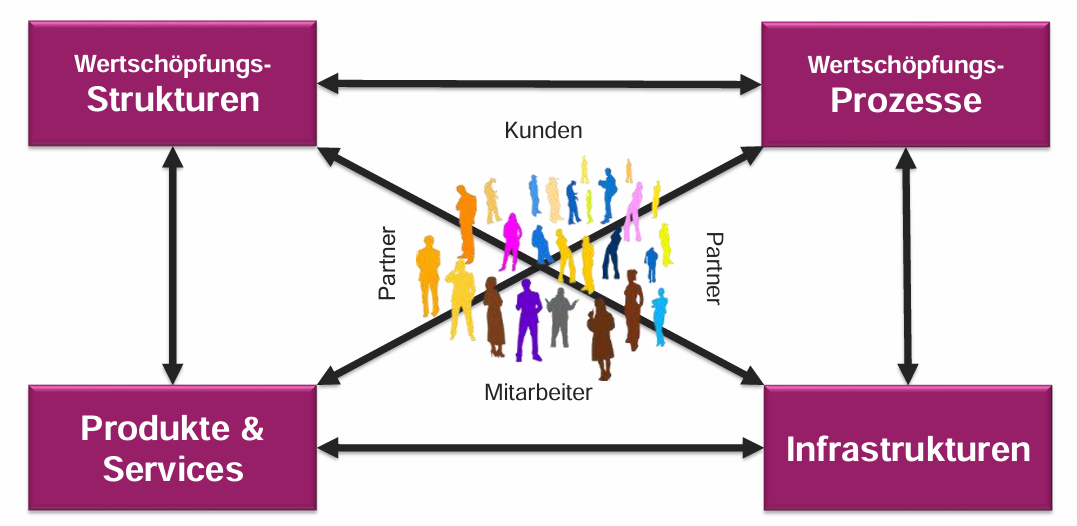
\includegraphics[width=1\linewidth]{Images/digbus/digeconomy.png}
    \caption{Digital Economy}
\end{figure}

\defn{Transaktionskostenökonomie}{
    Untersucht, welche Kosten bei der Durchführung 
    von wirtschaftlichen Transaktionen entstehen
    \begin{itemize}
        \item  Ex-ante Kosten: Diese entstehen vor der Transaktion
        \item Ex-post Kosten: Diese treten nach der Transaktion auf
    \end{itemize}
}
\begin{figure}[H]
    \centering
    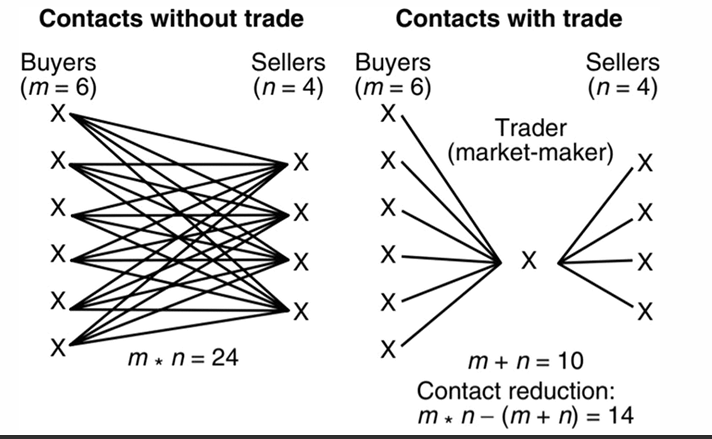
\includegraphics[width=1\linewidth]{Images/digbus/intermediation.png}
    \caption{Intermediation: bridging of incompatibilities between two (market) sides}
\end{figure}

Transaktionskosten:
Transaktionskosten sind:
\begin{itemize}
    \item Search costs
    \item Contracting costs
    \item Monitoring costs
    \item Adaption costs
\end{itemize}

\defn{Wertschöpfungsstrukturen}{
    \textbf{Dis-Intermediation}: Dekonstruktion von traditionellen 
    Wertschöpfungsketten, Eliminierung von traditionellen Mittlern
    , Direktzugriff der Käufer auf die Hersteller.

    \begin{itemize}
        \item displacement or elimination of market intermediaries
    \end{itemize}
    
    \textbf{Re-Intermediation}: Entwicklung neuer Wertschöpfungsketten/ -systeme
    , Neue (Online-) Intermediäre: Cybermediaries
}

\begin{figure}[H]
    \centering
    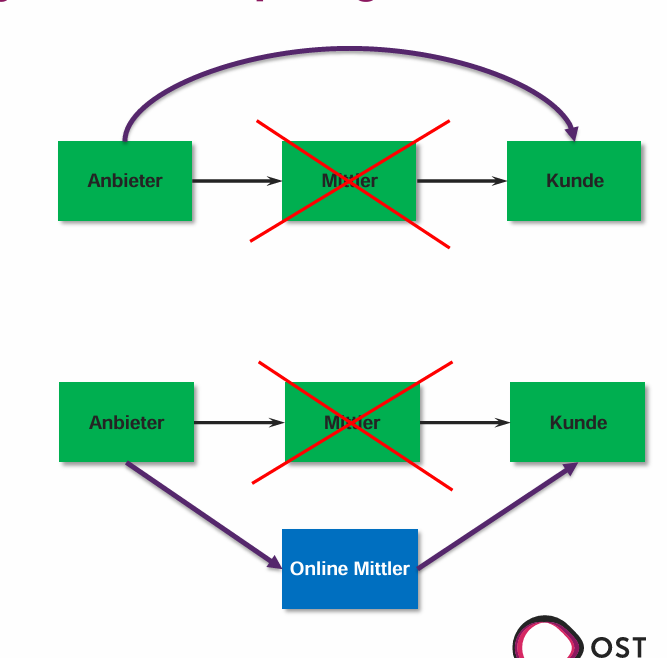
\includegraphics[width=1\linewidth]{Images/digbus/reintermediation.png}
    \caption{Reintermediation in der Digital Economy}
\end{figure}

\begin{figure}[H]
    \centering
    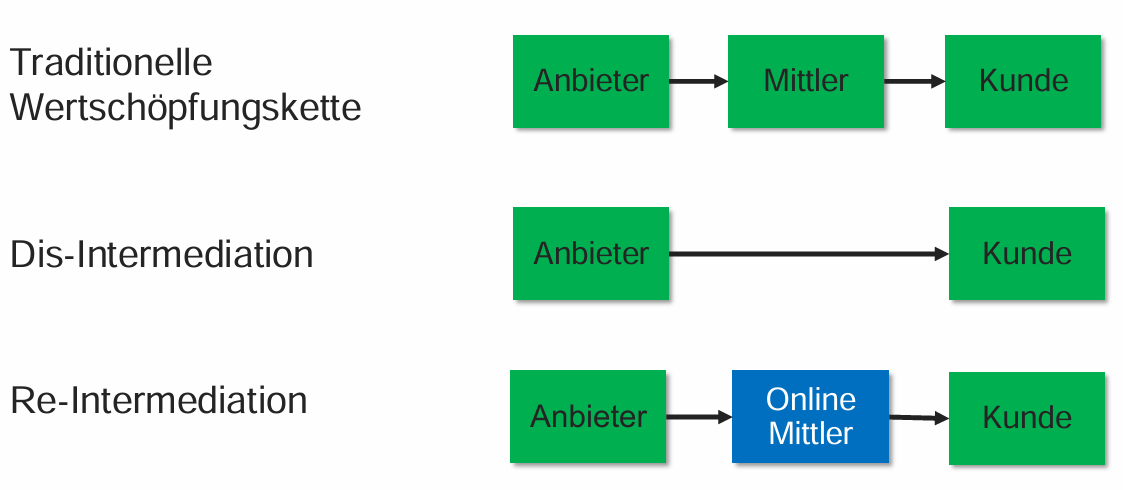
\includegraphics[width=1\linewidth]{Images/digbus/wertschoepfung.png}
    \caption{Wertschöpfungsstrukturen}
\end{figure}

\begin{figure}[H]
    \centering
    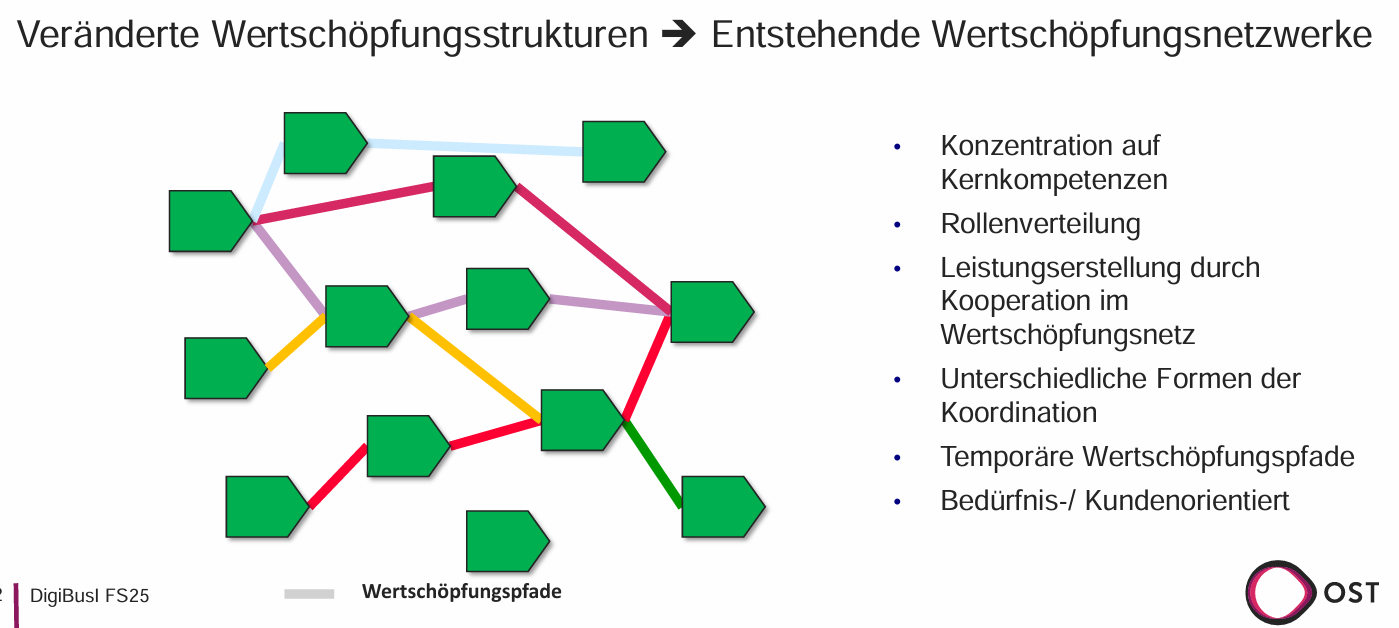
\includegraphics[width=1\linewidth]{Images/digbus/wertnetze.png}
    \caption{Wertschöpfungsnetzwerke: Die Kundenbedürfnisse 
    definieren das Wertschöpfungsnetz}
\end{figure}

\begin{figure}[H]
    \centering
    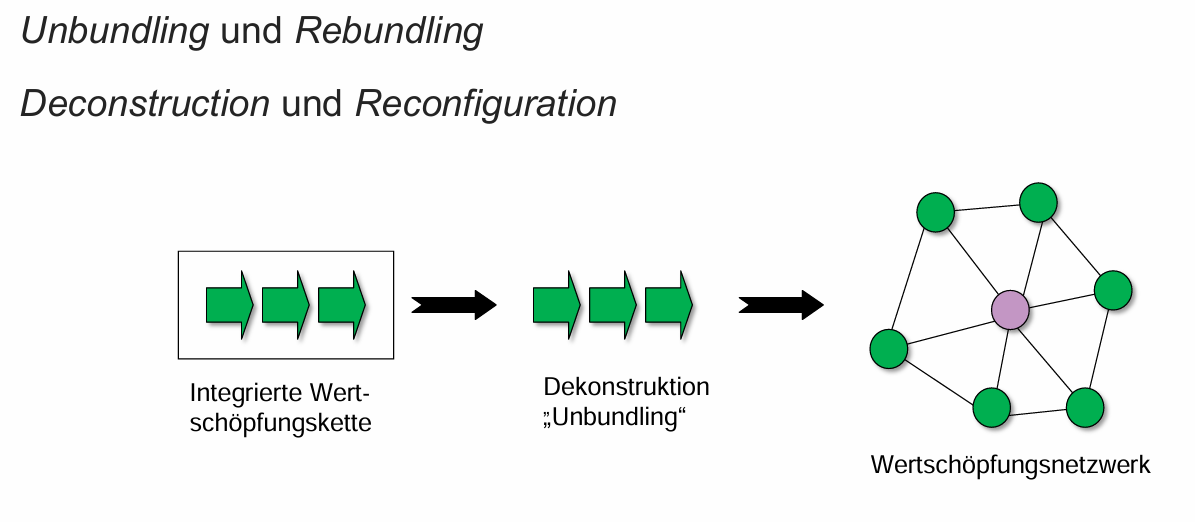
\includegraphics[width=1\linewidth]{Images/digbus/rebundling.png}
    \caption{Strategie zum Netzwerkbau}
\end{figure}

\subsection{Wertschöpfungsprozesse}
\defn{Wertschöpfungsprozesse}{
    \begin{enumerate}
        \item Interaktive Wertschöpfung: Open Innovation
            \begin{itemize}
                \item Statt sich nur auf die internen Fähigkeiten der 
                eigenen Forscher und Entwickler zu verlassen, werden externe Problemlöser in den 
                Innovationsprozess integriert. durch einen offenen Aufruf!
            \end{itemize}
        \item Interaktive Wertschöpfung: Mass Customization
        \item Der veränderte Kaufprozess
        \item Social Commerce
            \begin{itemize}
                \item Form des E-Commerce, die einen Kundenmehrwert 
                durch die aktive Einbindung der Kunden (User Generated Content) und deren 
                Vernetzung untereinander schafft.
            \end{itemize}
        \item Neue Formen von Produktionsprozessen
    \end{enumerate}
}

\begin{figure}[H]
    \centering
    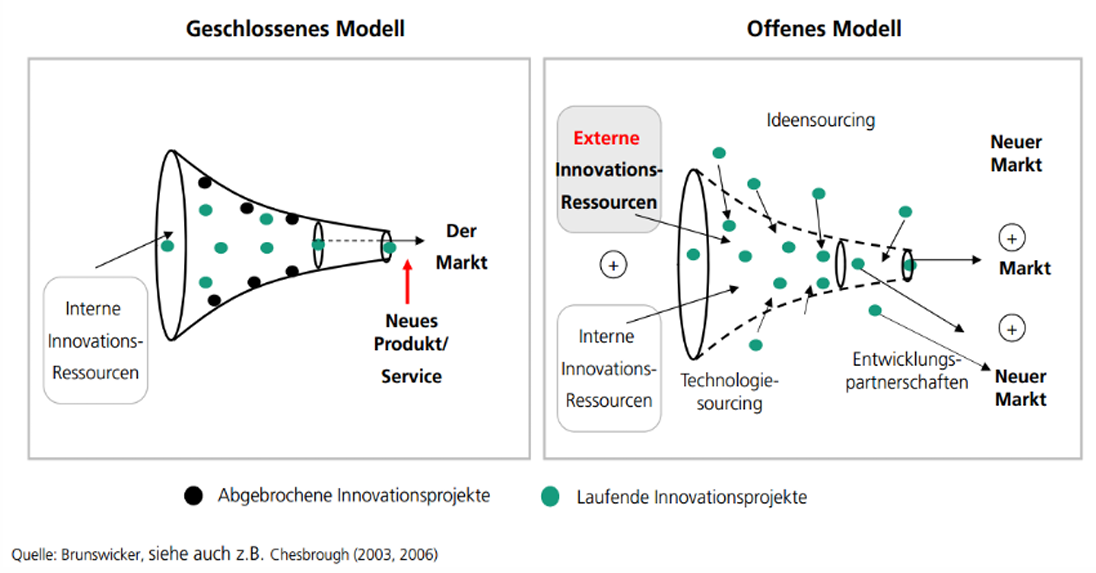
\includegraphics[width=1\linewidth]{Images/digbus/openinnovation.png}
    \caption{Open Innovation}
\end{figure}

\begin{figure}[H]
    \centering
    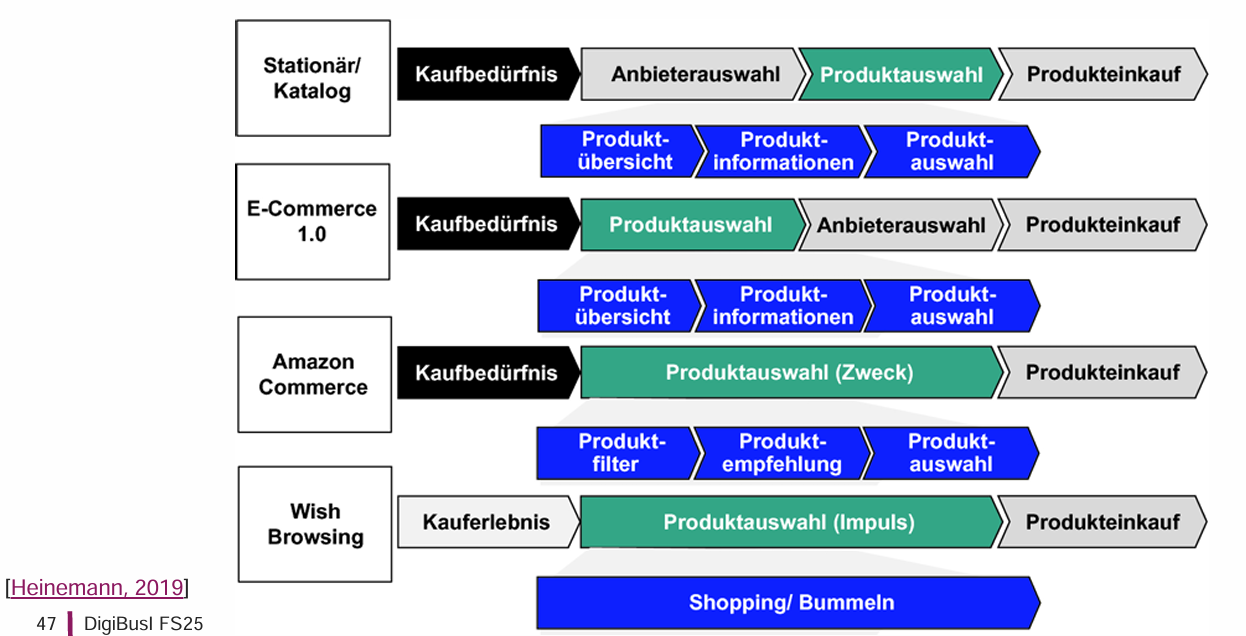
\includegraphics[width=1\linewidth]{Images/digbus/kaufprozess.png}
    \caption{Veränderung im Kaufprozess}
\end{figure}

\begin{figure}[H]
    \centering
    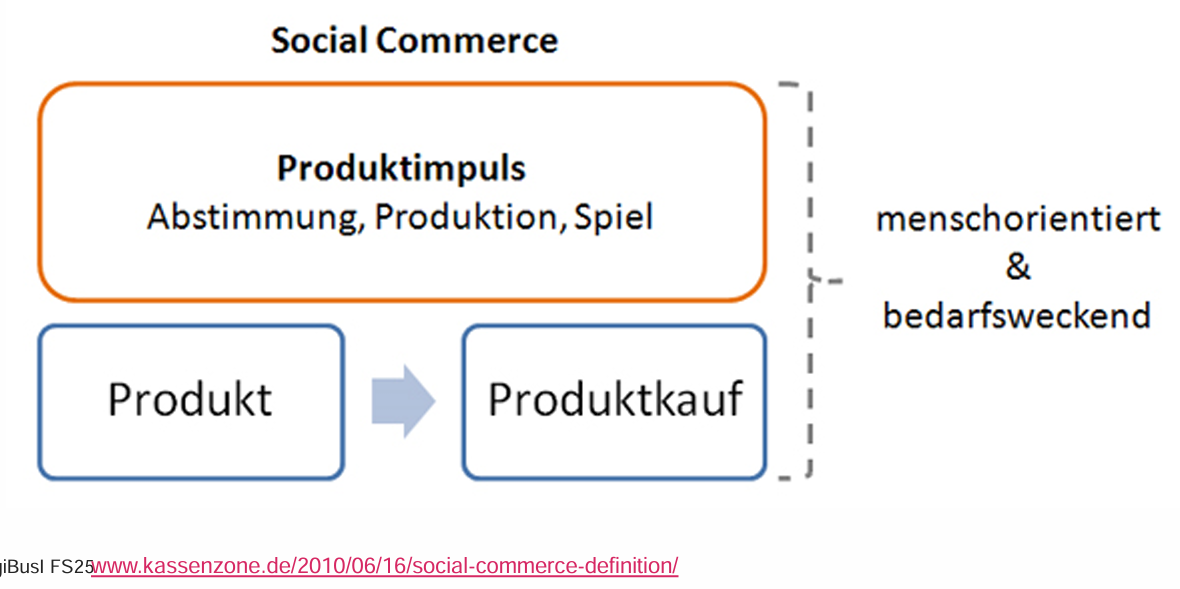
\includegraphics[width=1\linewidth]{Images/digbus/socialcomm.png}
    \caption{Social Commerce}
\end{figure}

\begin{figure}[H]
    \centering
    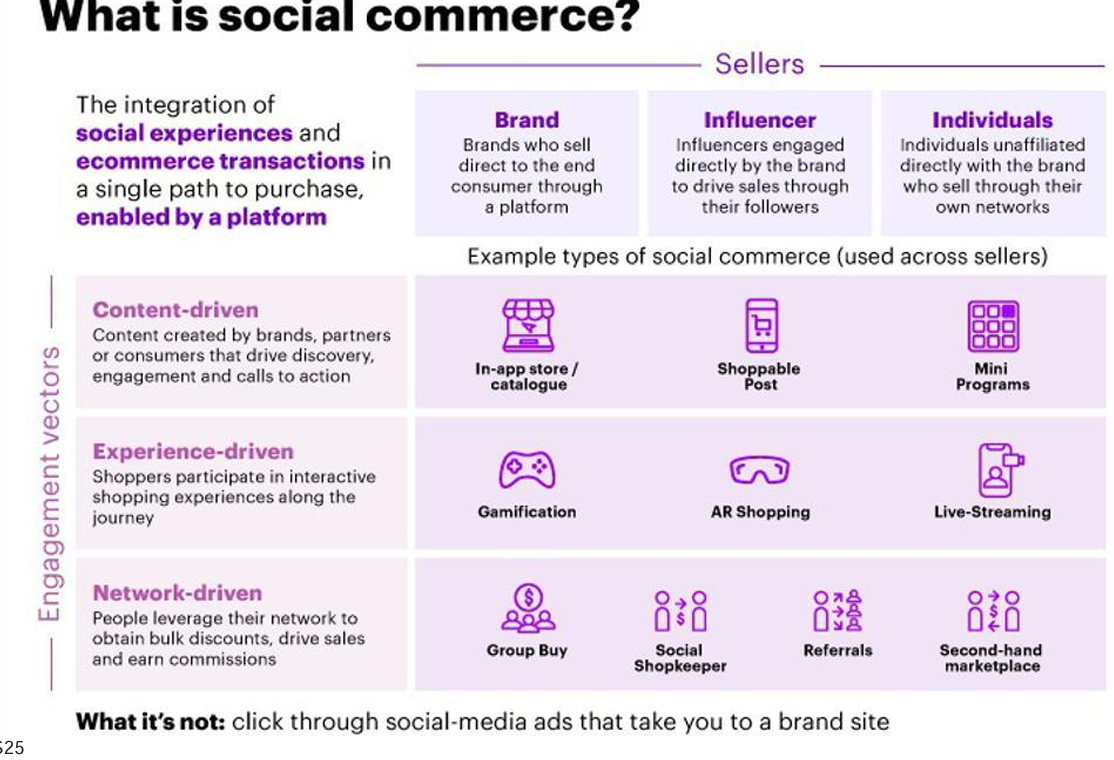
\includegraphics[width=1\linewidth]{Images/digbus/socialcommvec.png}
    \caption{Social Commerce Vectors}
\end{figure}

\defn{Neue Produktionsprozesse}{
    \begin{itemize}
        \item On-Demand Manufacturing
            \begin{itemize}
                \item Consumer-to-Manufacturer, C2M
            \end{itemize}
    \end{itemize}
}

\begin{figure}[H]
    \centering
    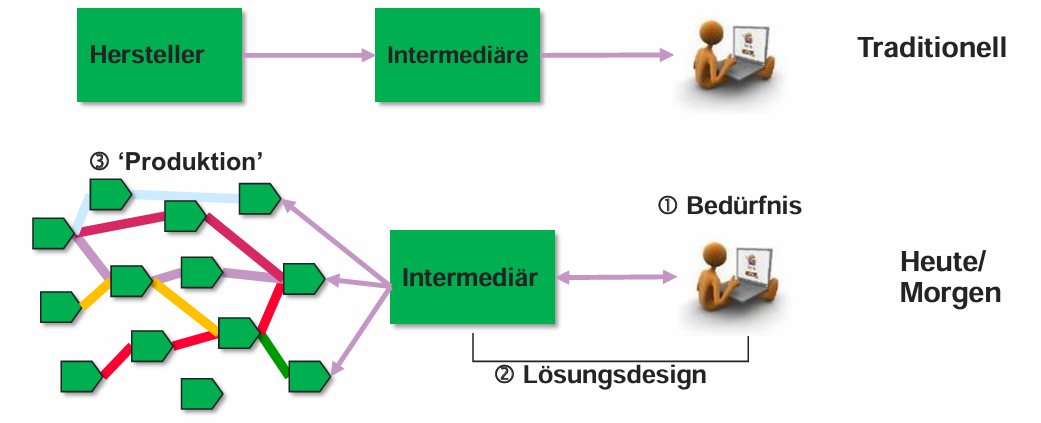
\includegraphics[width=1\linewidth]{Images/digbus/wertschzsm.png}
    \caption{Wertschöpfungsstrukturen und -prozesse}
\end{figure}

\section{Produkte und Services}
\defn{Produkte}{
    \begin{itemize}
        \item Flexible (Re-) Konfiguration digitaler Produkte
        \item Digitally charged products
            \begin{itemize}
                \item Erweiterung physischer Produkte mit digitalen Funktionen
                \item hybridity, smartness, connectivity, servitization and digitized product ecosystems.
            \end{itemize}
        \item Neue Services
    \end{itemize}
}

\defn{Services}{
    \begin{itemize}
        \item IFTTT (IF, Then Do)
        \item Mobility as a Service (MaaS)
        \item  LPaaS- Logistic Process as a Service
            \begin{itemize}
                \item Logistics Mall
            \end{itemize}
    \end{itemize}
}

\section{Digitale Plattformen und Ökosysteme}

\begin{figure}[H]
    \centering
    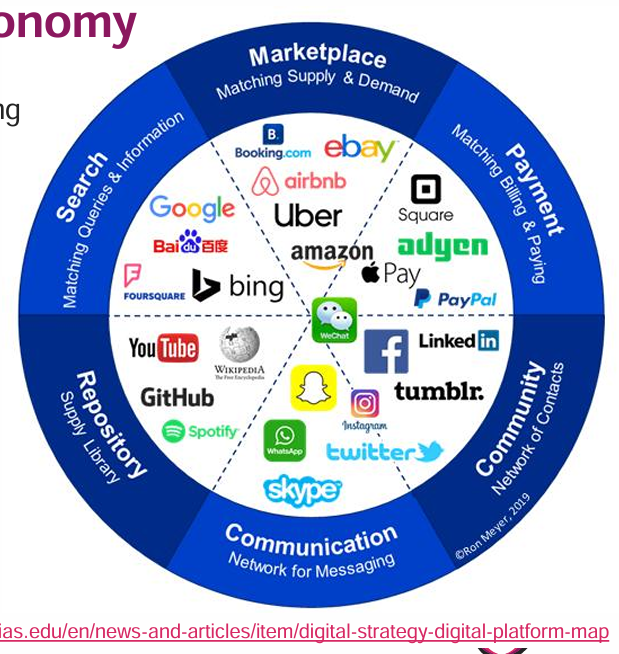
\includegraphics[width=1\linewidth]{Images/digbus/digplatmap.png}
    \caption{Digital Platform map}
\end{figure}

\defn{Digitale Platform}{
    \begin{itemize}
        \item Technologien oder Infrastrukturen, die die Interaktion zwischen 
        verschiedenen Nutzergruppen ermöglichen.
        \item Bieten eine zentrale Schnittstelle, über die verschiedene Akteure (z. B. Anbieter und 
        Nachfrager) miteinander in Kontakt treten können.
        \item  fungieren als Intermediäre, stellen die erforderliche Infrastruktur bereit und ermöglichen 
        unter vorgegebenen Regeln wertschaffende Interaktionen zwischen mindestens zwei 
        Akteuren, i. d. R. Anbieter und Kunden.
        \item wertschaffenden Interaktionen: Austausch von Informationen, Gütern 
        Dienstleistungen + Zahlungsmittel.
        \item
    \end{itemize}
}

Kernbestandteile:
\begin{itemize}
    \item Disintermediation und Re-Intermediation
    \item Netzwerkeffekte
    \item Plattform Governance
    \item Grundlage von Plattform-basierten Geschäftsmodellen
    \item Skalierbarkeit
    \item Datenzentriertheit
    \item Ökosysteme
    \item Innovationsfreundlichkeit
    \item Technologische Infrastruktur
\end{itemize}

\defn{Netzwerkeffekte}{
    Nutzen eines Gutes mit steigender Nutzerzahl (i.d.R.) 
    zunimmt (positive Netzwerkeffekte)
}

\begin{figure}[H]
    \centering
    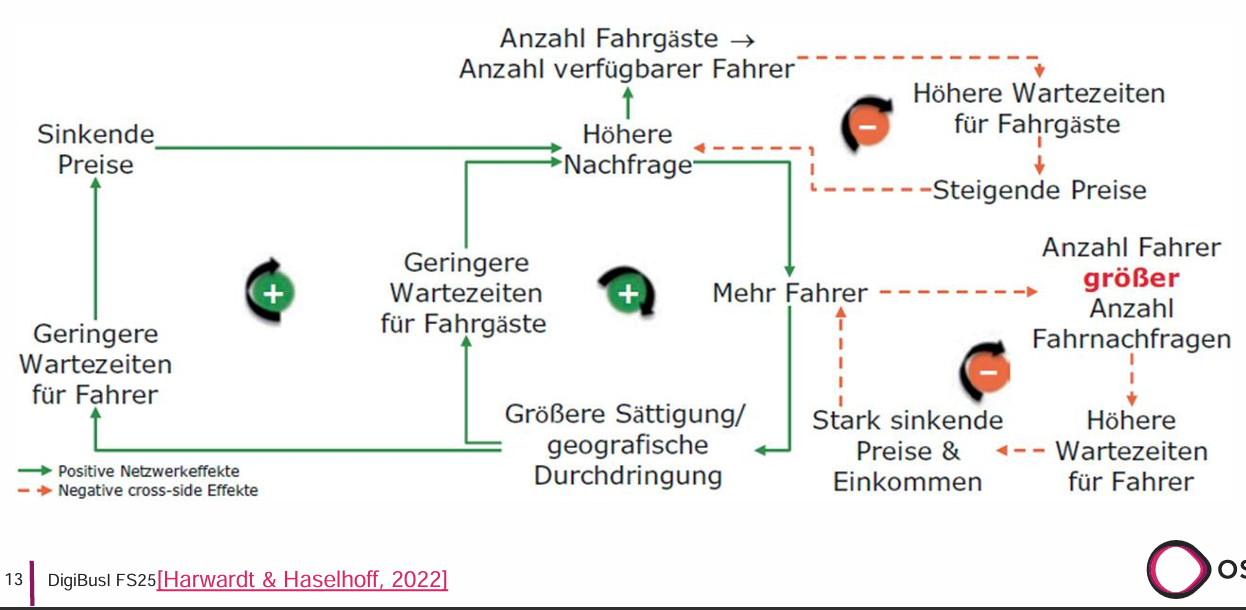
\includegraphics[width=1\linewidth]{Images/digbus/netzwerkeffekteuber.png}
    \caption{Netzwerkeffekte am Beispiel Uber}
\end{figure}

\begin{figure}[H]
    \centering
    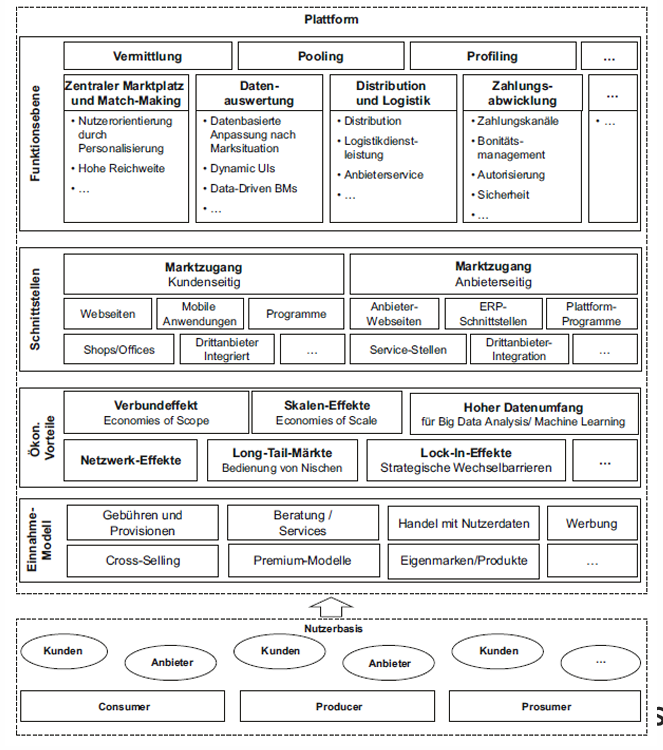
\includegraphics[width=1\linewidth]{Images/digbus/kernplattform.png}
    \caption{Kernbestandteile Plattform}
\end{figure}

\begin{figure}[H]
    \centering
    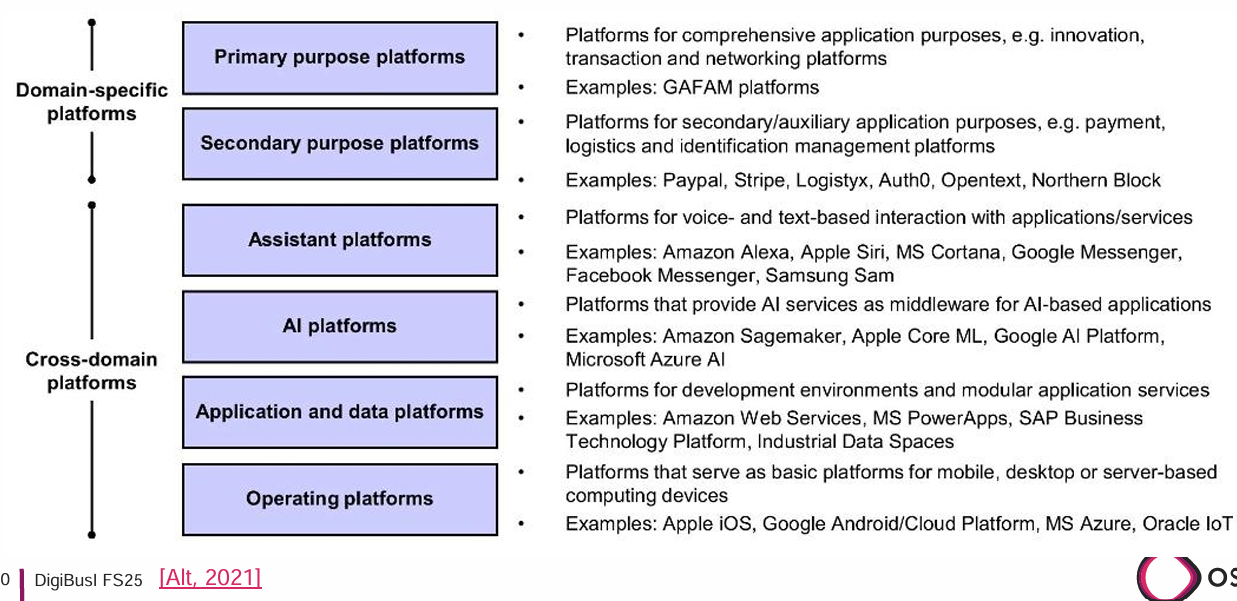
\includegraphics[width=1\linewidth]{Images/digbus/platformvar.png}
    \caption{Plattform Varianten}
\end{figure}

\begin{figure}[H]
    \centering
    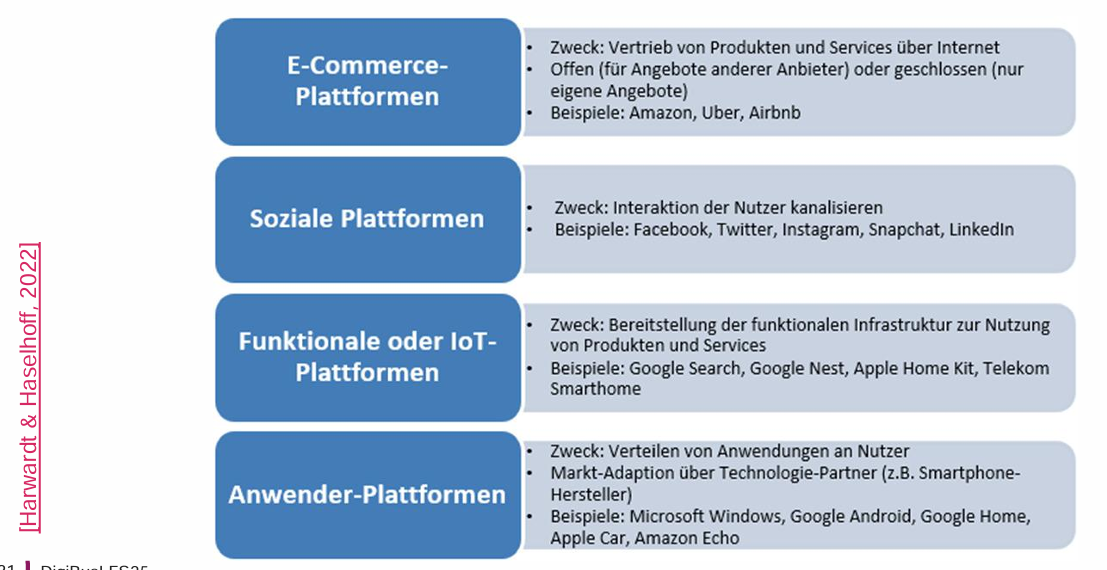
\includegraphics[width=1\linewidth]{Images/digbus/platformvar2.png}
    \caption{Plattform Varianten}
\end{figure}

Weg zur Platformökonomie:
\begin{enumerate}
    \item Von der Ressourcen-Kontrolle zur Ressourcen-„Orchestrierung“
    \item Von der internen Optimierung zur externen Interaktion
    \item Veränderung 3: Vom Fokus auf Kundenwert auf den Fokus auf Ökosystem-Wert
\end{enumerate}

\defn{Digital Ecosystem}{
    Ein Digitales Ökosystem ist ein sozio-technisches System, in dem Unternehmen und 
    Menschen kooperieren, die zwar unabhängig sind, sich von der Teilnahme aber einen 
    gegenseitigen Vorteil versprechen. 
    Ein Digitales Ökosystem hat in seinem Zentrum eine digitale Plattform.
}

\section{ Geschäftsmodelle im Digital Business}

\begin{figure}[H]
    \centering
    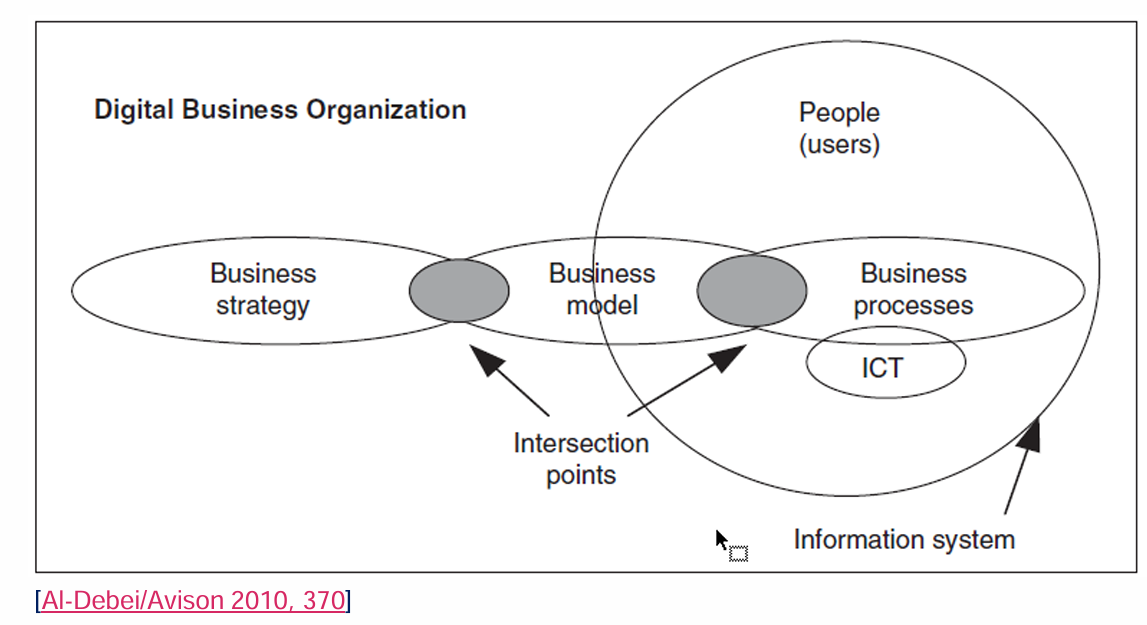
\includegraphics[width=1\linewidth]{Images/digbus/stratproc.png}
    \caption{Von Strategie zum Prozess}
\end{figure}

\begin{figure}[H]
    \centering
    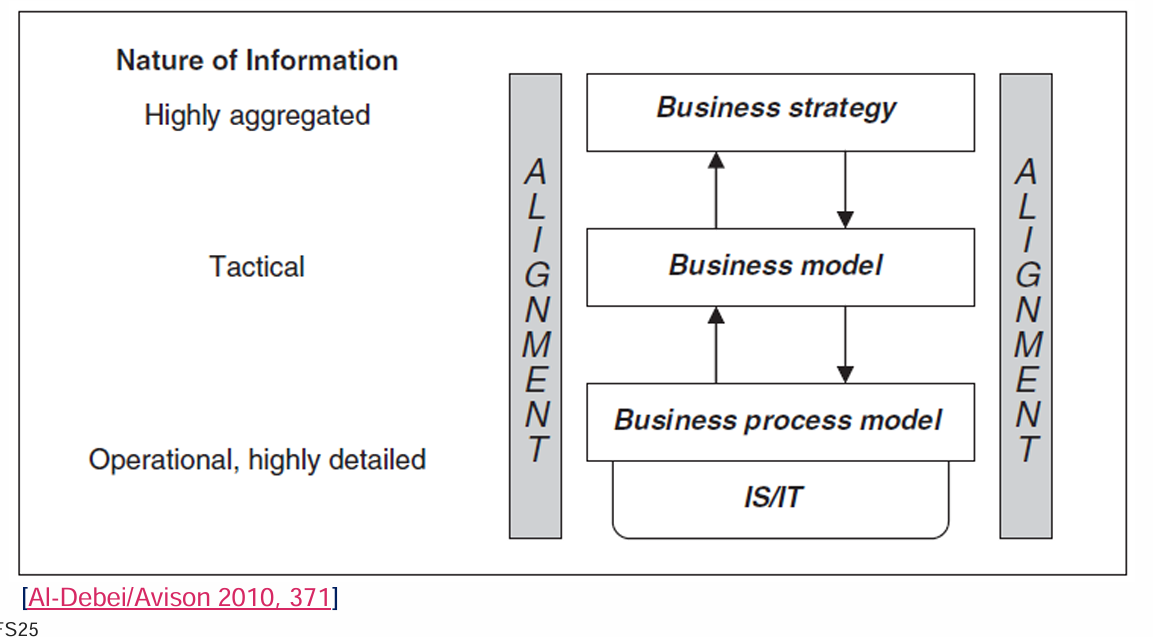
\includegraphics[width=1\linewidth]{Images/digbus/stratproc2.png}
    \caption{Von Strategie zum Prozess: Top Down View}
\end{figure}

\defn{Business Model}{
    Geschäftsmodelle können als das fehlende Bindeglied zwischen Strategie und Geschäfts
    prozessen oder als Bindeglied zwischen der Planungs- und der Umsetzungsebene eines 
    Unternehmens gesehen werden.

    \begin{itemize}
        \item Geschäftsmodelle kommen, insbesondere in IT-getriebenen und digitalen Unternehmen, als 
        Werkzeug für die Abbildung, Innovation und Evaluation der Geschäftslogik zum Einsatz.
    \end{itemize}

    Nutzen:
    \begin{itemize}
        \item Understand and share
        \item Analyze
        \item Manage 
        \item Prospect
    \end{itemize}
}

\begin{figure}[H]
    \centering
    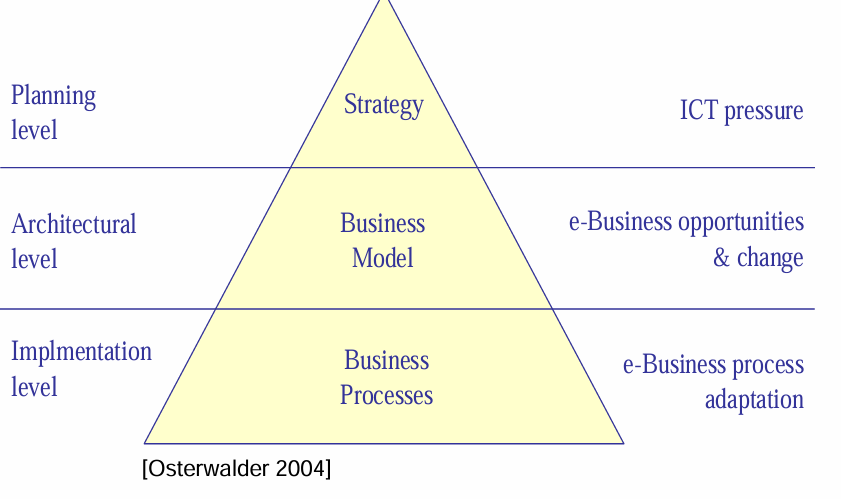
\includegraphics[width=1\linewidth]{Images/digbus/model.png}
    \caption{Eingliederung des Business Model}
\end{figure}

\defn{Geschäftsmodell Logik}{
    Ein Geschäftsmodell spiegelt die 
    innere Logik des Unternehmens 
    wider: 
    Es beschreibt, welcher Nutzen für 
    den Kunden erbracht wird und wie 
    damit Geld verdient werden soll. 
    Dabei kommt dem Kundennutzen
    eine hohe Bedeutung zu.
}

\begin{figure}[H]
    \centering
    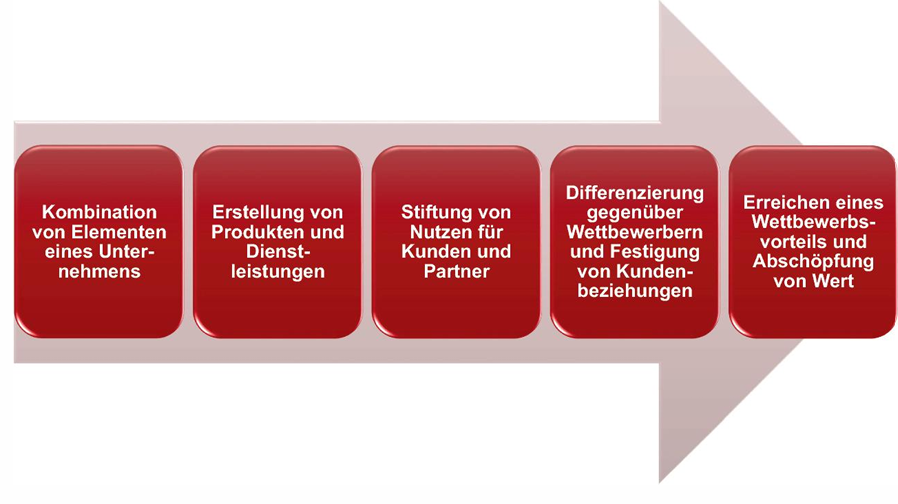
\includegraphics[width=1\linewidth]{Images/digbus/modellogic.png}
    \caption{Business Model Logic}
\end{figure}

Interlocking Elements:
\begin{itemize}
    \item Customer value proposition (CVP)
    \item Profit formula
        \begin{itemize}
            \item Revenue model, Cost structure, Margin model, Resource velocity
        \end{itemize}
    \item Key resources
    \item Key  processes
\end{itemize}
These four elements form the building blocks of any business.

\begin{figure}[H]
    \centering
    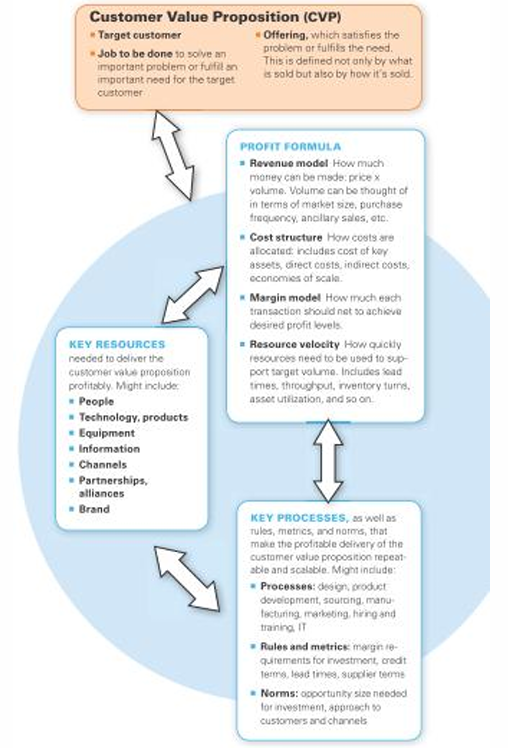
\includegraphics[width=1\linewidth]{Images/digbus/modelelements.png}
    \caption{Business Model Elements}
\end{figure}

\defn{Digital Business Model}{
    basierend auf elektronischen Wertschöpfungsprozessen 
    als zentraler Punkt ihrer Geschäftsstrategie und 
    somit als Treiber ihres Wettbewerbsvorteils.
    \begin{itemize}
        \item  Logik, wie ein Unternehmen 
            innerhalb der Net Economy agiert und wie es nachhaltig Wert schafft durch elektronische, 
            informationsbezogene Prozesse basierend auf und ermöglicht durch innovative 
            Informationstechnologie
        \item Wertschöpfung digital
        \item Neuartige Geschäftsmodelle
        \item Rekonfiguration bestehender Geschäftsmodelle
    \end{itemize}
}

\begin{figure}[H]
    \centering
    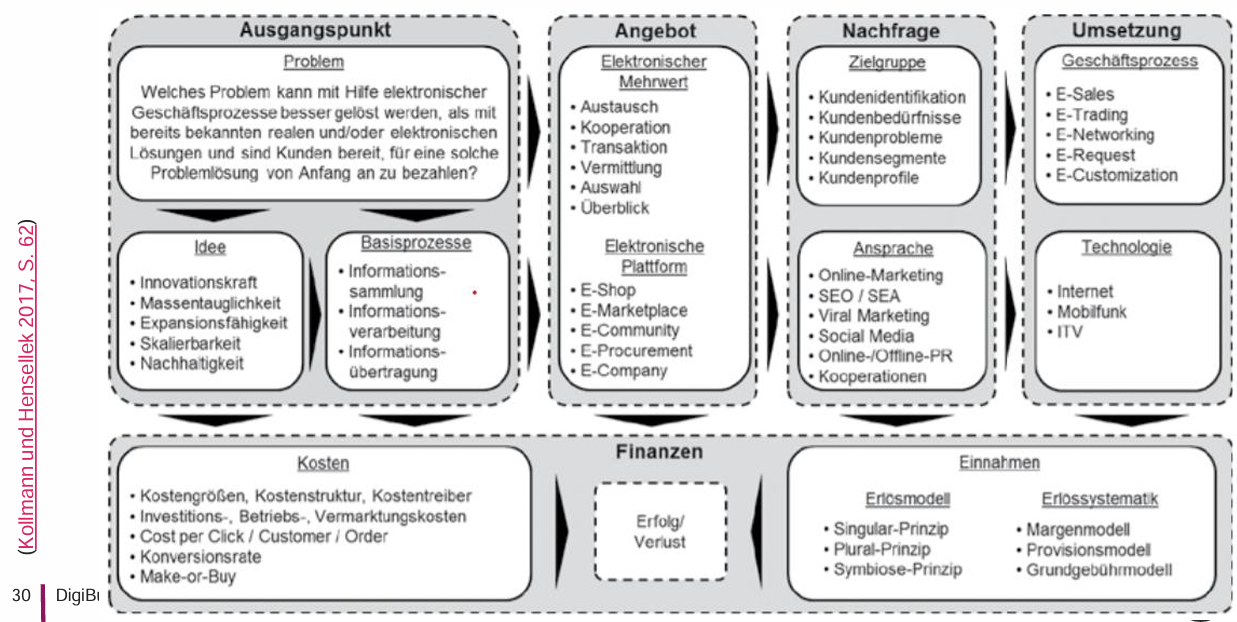
\includegraphics[width=1\linewidth]{Images/digbus/digmodarch.png}
    \caption{Basis Architektur digitaler Geschäftsmodelle}
\end{figure}

\begin{figure}[H]
    \centering
    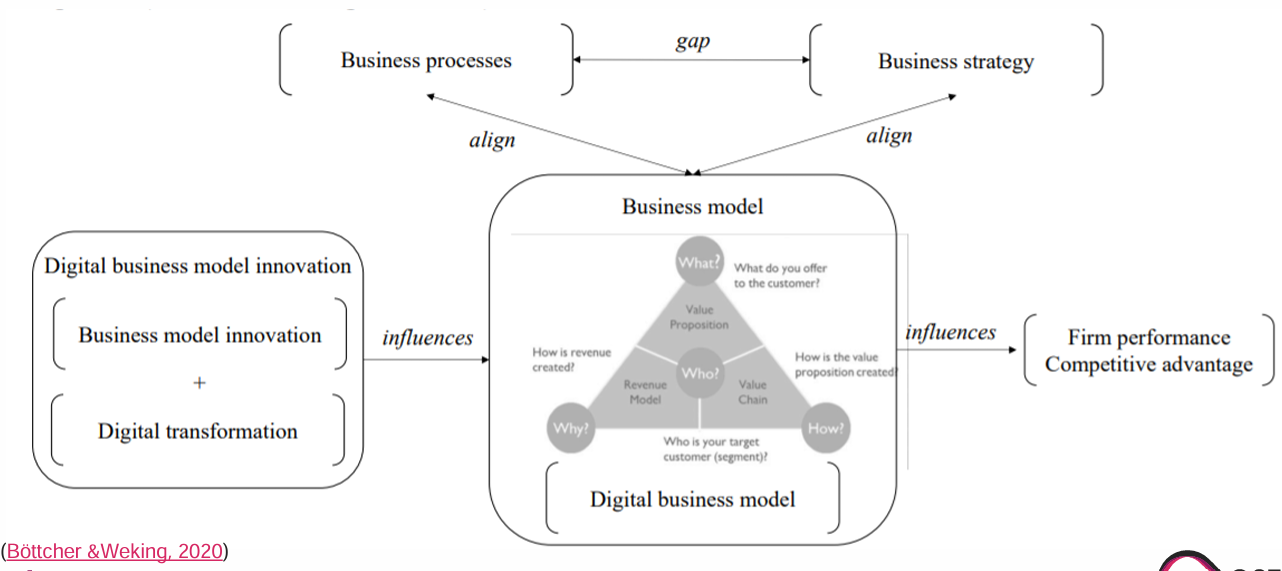
\includegraphics[width=1\linewidth]{Images/digbus/modeldesign.png}
    \caption{Digital Model Design}
\end{figure}
\begin{figure}[H]
    \centering
    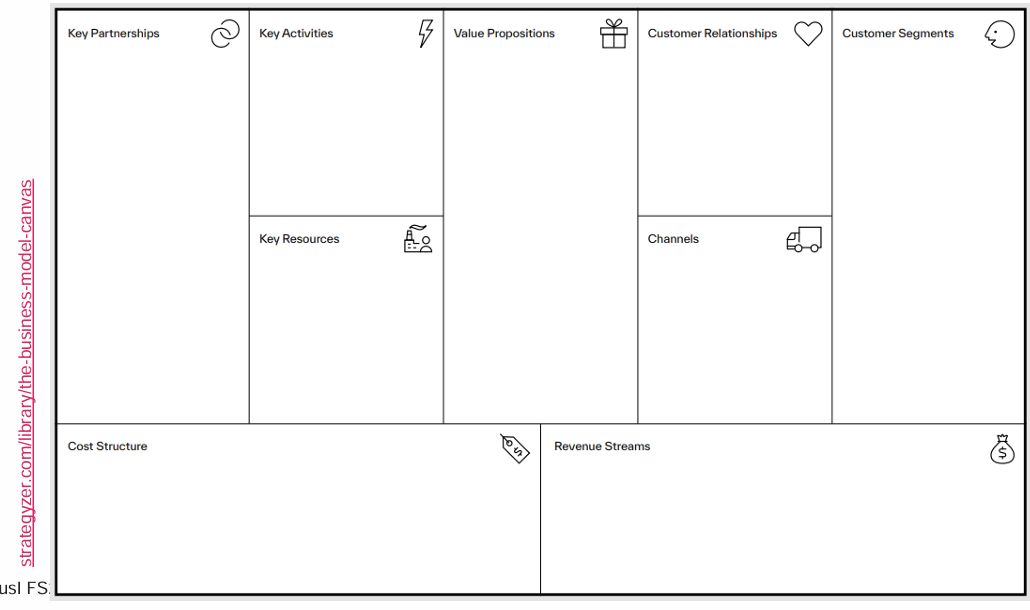
\includegraphics[width=1\linewidth]{Images/digbus/modeldesigncanvas.png}
    \caption{Digital Model Design}
\end{figure}
\begin{figure}[H]
    \centering
    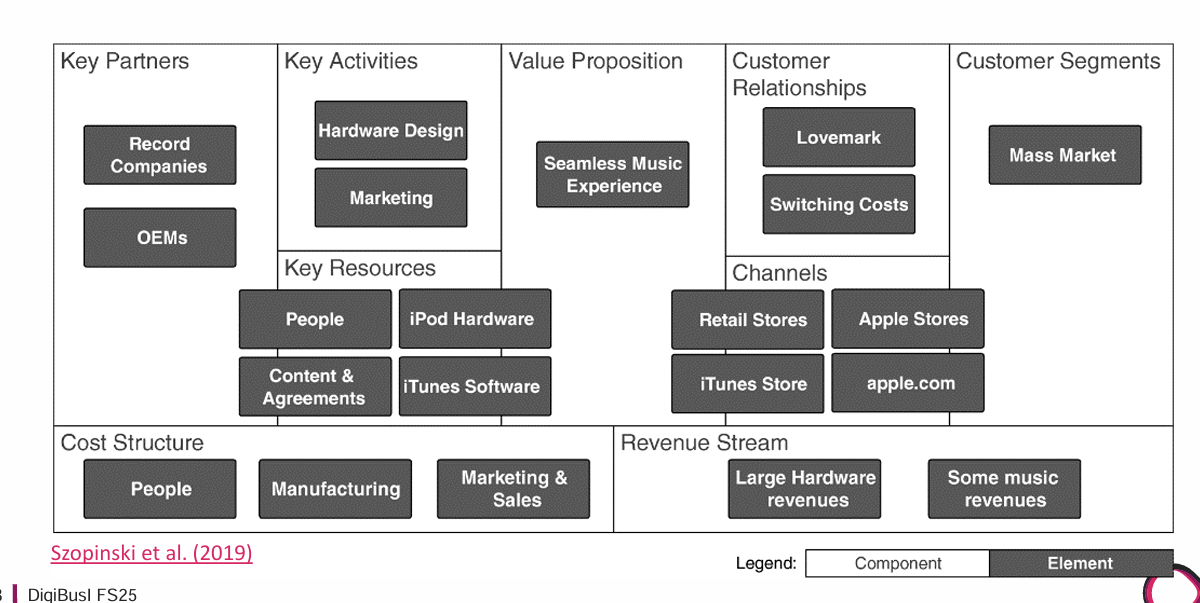
\includegraphics[width=1\linewidth]{Images/digbus/modeldesignexample.png}
    \caption{Digital Model Design Example}
\end{figure}
\begin{figure}[H]
    \centering
    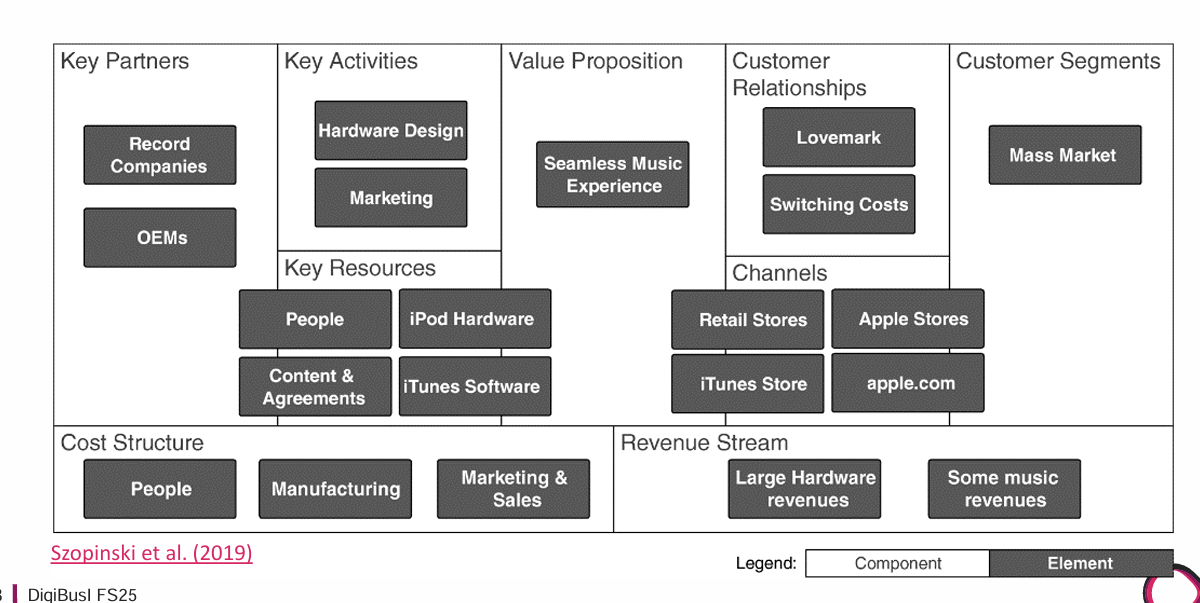
\includegraphics[width=1\linewidth]{Images/digbus/modeldesignexample.png}
    \caption{Digital Model Navigator}
\end{figure}

Arten:
\begin{itemize}
    \item Subscription
    \item Razor and Blade (Haken und Köder)
    \item Freemium
    \item Advertisement
    \item https://businessmodelnavigator.com/explore
    \item https://www.linkedin.com/pulse/teil-2-st-gallener-business-model-navigator-christian-hoffmeister/
\end{itemize}

\end{document}
